% Options for packages loaded elsewhere
\PassOptionsToPackage{unicode}{hyperref}
\PassOptionsToPackage{hyphens}{url}
\PassOptionsToPackage{dvipsnames,svgnames,x11names}{xcolor}
%
\documentclass[
  letterpaper,
  DIV=11,
  numbers=noendperiod]{scrartcl}

\usepackage{amsmath,amssymb}
\usepackage{lmodern}
\usepackage{iftex}
\ifPDFTeX
  \usepackage[T1]{fontenc}
  \usepackage[utf8]{inputenc}
  \usepackage{textcomp} % provide euro and other symbols
\else % if luatex or xetex
  \usepackage{unicode-math}
  \defaultfontfeatures{Scale=MatchLowercase}
  \defaultfontfeatures[\rmfamily]{Ligatures=TeX,Scale=1}
\fi
% Use upquote if available, for straight quotes in verbatim environments
\IfFileExists{upquote.sty}{\usepackage{upquote}}{}
\IfFileExists{microtype.sty}{% use microtype if available
  \usepackage[]{microtype}
  \UseMicrotypeSet[protrusion]{basicmath} % disable protrusion for tt fonts
}{}
\makeatletter
\@ifundefined{KOMAClassName}{% if non-KOMA class
  \IfFileExists{parskip.sty}{%
    \usepackage{parskip}
  }{% else
    \setlength{\parindent}{0pt}
    \setlength{\parskip}{6pt plus 2pt minus 1pt}}
}{% if KOMA class
  \KOMAoptions{parskip=half}}
\makeatother
\usepackage{xcolor}
\setlength{\emergencystretch}{3em} % prevent overfull lines
\setcounter{secnumdepth}{-\maxdimen} % remove section numbering
% Make \paragraph and \subparagraph free-standing
\ifx\paragraph\undefined\else
  \let\oldparagraph\paragraph
  \renewcommand{\paragraph}[1]{\oldparagraph{#1}\mbox{}}
\fi
\ifx\subparagraph\undefined\else
  \let\oldsubparagraph\subparagraph
  \renewcommand{\subparagraph}[1]{\oldsubparagraph{#1}\mbox{}}
\fi


\providecommand{\tightlist}{%
  \setlength{\itemsep}{0pt}\setlength{\parskip}{0pt}}\usepackage{longtable,booktabs,array}
\usepackage{calc} % for calculating minipage widths
% Correct order of tables after \paragraph or \subparagraph
\usepackage{etoolbox}
\makeatletter
\patchcmd\longtable{\par}{\if@noskipsec\mbox{}\fi\par}{}{}
\makeatother
% Allow footnotes in longtable head/foot
\IfFileExists{footnotehyper.sty}{\usepackage{footnotehyper}}{\usepackage{footnote}}
\makesavenoteenv{longtable}
\usepackage{graphicx}
\makeatletter
\def\maxwidth{\ifdim\Gin@nat@width>\linewidth\linewidth\else\Gin@nat@width\fi}
\def\maxheight{\ifdim\Gin@nat@height>\textheight\textheight\else\Gin@nat@height\fi}
\makeatother
% Scale images if necessary, so that they will not overflow the page
% margins by default, and it is still possible to overwrite the defaults
% using explicit options in \includegraphics[width, height, ...]{}
\setkeys{Gin}{width=\maxwidth,height=\maxheight,keepaspectratio}
% Set default figure placement to htbp
\makeatletter
\def\fps@figure{htbp}
\makeatother
\newlength{\cslhangindent}
\setlength{\cslhangindent}{1.5em}
\newlength{\csllabelwidth}
\setlength{\csllabelwidth}{3em}
\newlength{\cslentryspacingunit} % times entry-spacing
\setlength{\cslentryspacingunit}{\parskip}
\newenvironment{CSLReferences}[2] % #1 hanging-ident, #2 entry spacing
 {% don't indent paragraphs
  \setlength{\parindent}{0pt}
  % turn on hanging indent if param 1 is 1
  \ifodd #1
  \let\oldpar\par
  \def\par{\hangindent=\cslhangindent\oldpar}
  \fi
  % set entry spacing
  \setlength{\parskip}{#2\cslentryspacingunit}
 }%
 {}
\usepackage{calc}
\newcommand{\CSLBlock}[1]{#1\hfill\break}
\newcommand{\CSLLeftMargin}[1]{\parbox[t]{\csllabelwidth}{#1}}
\newcommand{\CSLRightInline}[1]{\parbox[t]{\linewidth - \csllabelwidth}{#1}\break}
\newcommand{\CSLIndent}[1]{\hspace{\cslhangindent}#1}

\KOMAoption{captions}{tableheading}
\makeatletter
\makeatother
\makeatletter
\makeatother
\makeatletter
\@ifpackageloaded{caption}{}{\usepackage{caption}}
\AtBeginDocument{%
\ifdefined\contentsname
  \renewcommand*\contentsname{Table of contents}
\else
  \newcommand\contentsname{Table of contents}
\fi
\ifdefined\listfigurename
  \renewcommand*\listfigurename{List of Figures}
\else
  \newcommand\listfigurename{List of Figures}
\fi
\ifdefined\listtablename
  \renewcommand*\listtablename{List of Tables}
\else
  \newcommand\listtablename{List of Tables}
\fi
\ifdefined\figurename
  \renewcommand*\figurename{Figure}
\else
  \newcommand\figurename{Figure}
\fi
\ifdefined\tablename
  \renewcommand*\tablename{Table}
\else
  \newcommand\tablename{Table}
\fi
}
\@ifpackageloaded{float}{}{\usepackage{float}}
\floatstyle{ruled}
\@ifundefined{c@chapter}{\newfloat{codelisting}{h}{lop}}{\newfloat{codelisting}{h}{lop}[chapter]}
\floatname{codelisting}{Listing}
\newcommand*\listoflistings{\listof{codelisting}{List of Listings}}
\makeatother
\makeatletter
\@ifpackageloaded{caption}{}{\usepackage{caption}}
\@ifpackageloaded{subcaption}{}{\usepackage{subcaption}}
\makeatother
\makeatletter
\@ifpackageloaded{tcolorbox}{}{\usepackage[many]{tcolorbox}}
\makeatother
\makeatletter
\@ifundefined{shadecolor}{\definecolor{shadecolor}{rgb}{.97, .97, .97}}
\makeatother
\makeatletter
\makeatother
\ifLuaTeX
  \usepackage{selnolig}  % disable illegal ligatures
\fi
\IfFileExists{bookmark.sty}{\usepackage{bookmark}}{\usepackage{hyperref}}
\IfFileExists{xurl.sty}{\usepackage{xurl}}{} % add URL line breaks if available
\urlstyle{same} % disable monospaced font for URLs
\hypersetup{
  pdftitle={Prodiges et vertiges des données satellitaires pour l'évaluation},
  pdfauthor={Florent Bédécarrats (IRD-SOURCE)},
  colorlinks=true,
  linkcolor={blue},
  filecolor={Maroon},
  citecolor={Blue},
  urlcolor={Blue},
  pdfcreator={LaTeX via pandoc}}

\title{Prodiges et vertiges des données satellitaires pour l'évaluation}
\author{\texttt{Florent\ Bédécarrats\ (IRD-SOURCE)}}
\date{}

\begin{document}
\maketitle
\ifdefined\Shaded\renewenvironment{Shaded}{\begin{tcolorbox}[boxrule=0pt, breakable, frame hidden, borderline west={3pt}{0pt}{shadecolor}, interior hidden, enhanced, sharp corners]}{\end{tcolorbox}}\fi

\hypertarget{objectifs-de-la-pruxe9sentation}{%
\subsection{Objectifs de la
présentation}\label{objectifs-de-la-pruxe9sentation}}

\begin{itemize}
\item
  Décrire la diversification des usages
\item
  Facteurs de diffusion
\item
  Risques associés
\item
  Solutions et précautions
\end{itemize}

\hypertarget{perspective}{%
\subsection{Perspective}\label{perspective}}

\begin{itemize}
\item
  Témoin et complice de l'adoption (AFD, KfW)
\item
  Laboratoire SOURCE
\item
  Agenda de recherche

  \begin{itemize}
  \tightlist
  \item
    Innovation sur les méthodes d'évaluation
  \item
    Application à des enjeux d'adaptation
  \item
    Economie politique de la mesure
  \end{itemize}
\end{itemize}

\hypertarget{exemple-irrigation-agricole}{%
\subsection{Exemple : irrigation
agricole}\label{exemple-irrigation-agricole}}

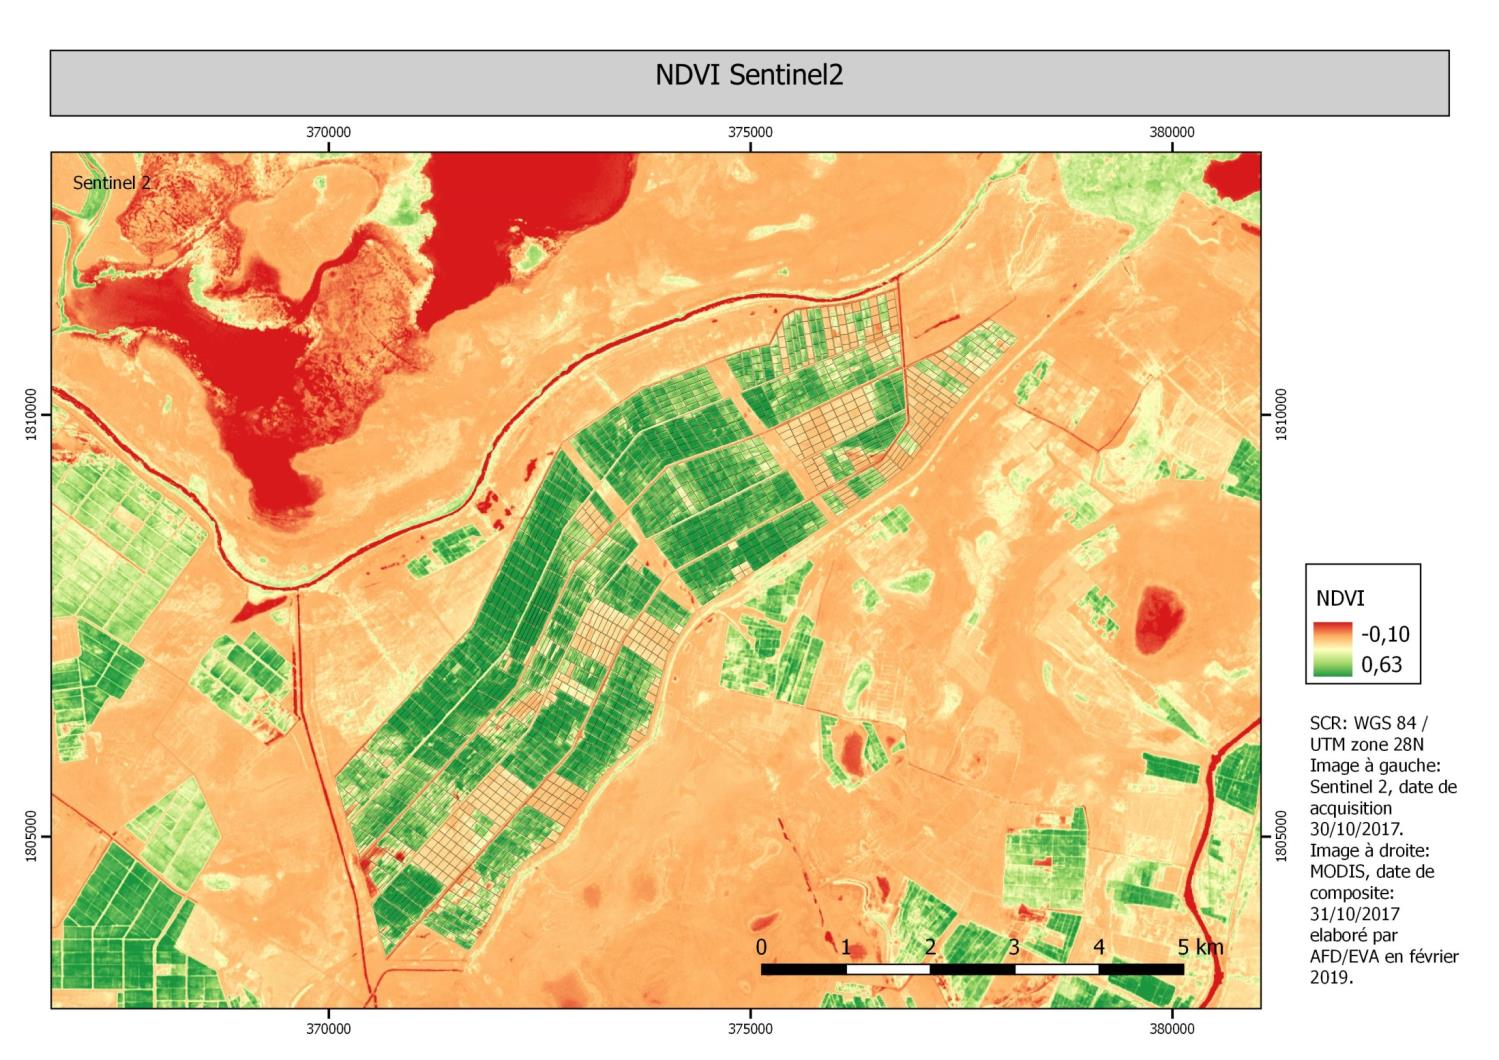
\includegraphics{sources/SAED_Agro.jpg}

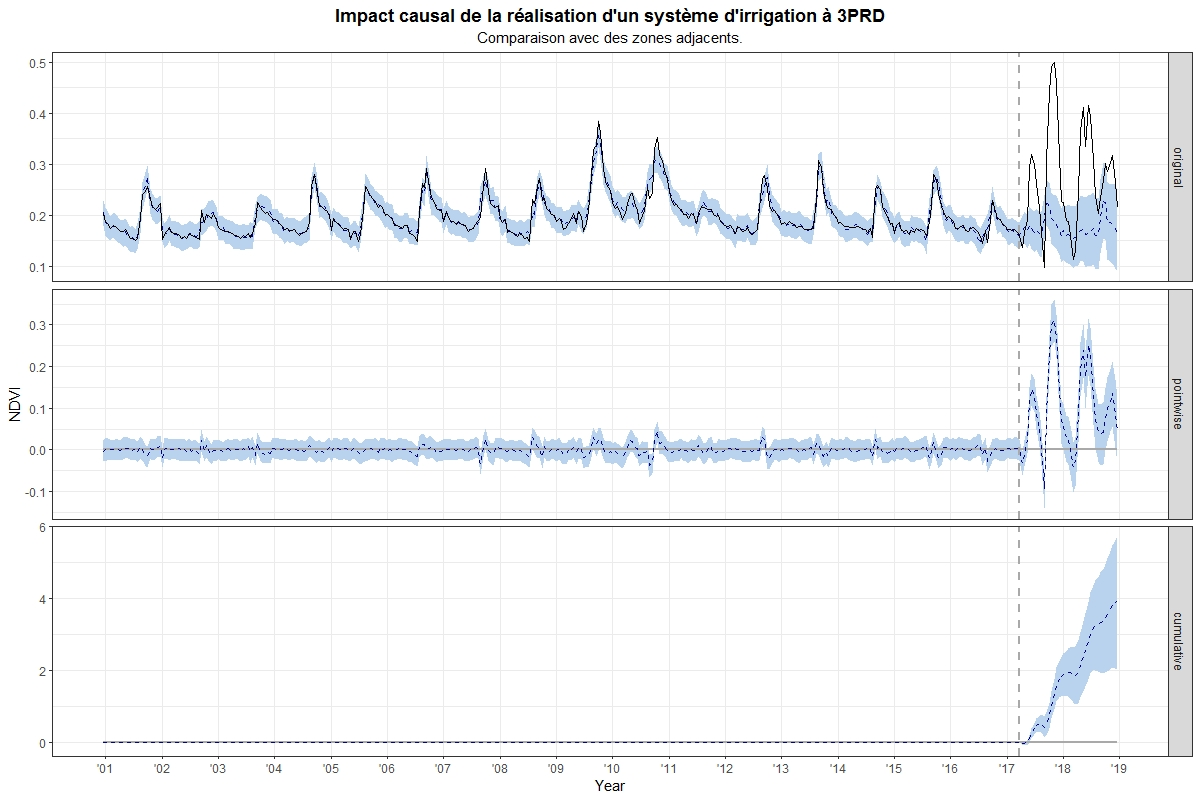
\includegraphics[width=6.25in,height=\textheight]{sources/SAED_Stats.jpg}

\hypertarget{diffusion-des-usages}{%
\subsection{Diffusion des usages}\label{diffusion-des-usages}}

\begin{itemize}
\item
  \textbf{Versant méthodologique}

  \begin{itemize}
  \tightlist
  \item
    Des sciences naturelles aux sciences sociales
  \item
    Du fondamental aux applications
  \end{itemize}
\item
  \textbf{Versant de la mise en oeuvre}

  \begin{itemize}
  \tightlist
  \item
    Evaluation ex post
  \item
    Suivi-évaluation
  \item
    Conception
  \item
    Opérationnel
  \end{itemize}
\end{itemize}

\hypertarget{champ-toujours-plus-large}{%
\subsection{Champ toujours plus large}\label{champ-toujours-plus-large}}

Quelques synthèses de la littérature en économie (Donaldson and
Storeygard 2016)

Les sujets ``classiques''

\begin{itemize}
\tightlist
\item
  Environnement/biodiversité
\item
  Gestion forestière, Qualité de l'air
\item
  Climat, météorologie
\item
  Topographie : accidenté
\item
  Agriculture, sécurité alimentaire
\item
  Hydrologie, risques naturels
\end{itemize}

``Nouveaux'' sujets

\begin{itemize}
\tightlist
\item
  Développement économique : luminosité, infrastructures
\item
  Urbanisation, bâti, localisation et mouvements de population,
  transports
\item
  Déterminants de santé
\item
  Raffinement des sujets classiques (ex. dégradation des forêts)
\item
  Interfaces entre ces sujets (``nexus'')
\end{itemize}

Les données satellitaires sont mobilisées pour calculer 30/231
indicateurs ODD et elles renseignent utilsement 71 des 169 cibles ODD
(GEO 2019; Estoque 2020).

\hypertarget{relation-aux-autres-sources}{%
\subsection{Relation aux autres
sources}\label{relation-aux-autres-sources}}

Besoins de croisement

\begin{itemize}
\tightlist
\item
  Relevés sur le terrain
\item
  Données administratives
\item
  Données crowdsourcées
\item
  Fusion de données : pauvreté, biodiversité, densité de population
\end{itemize}

\hypertarget{exemple-de-fusion-de-donnuxe9es}{%
\subsection{Exemple de fusion de
données}\label{exemple-de-fusion-de-donnuxe9es}}

Cartes de pauvreté (Lee and Braithwaite 2022)

Combinent des données :

\begin{itemize}
\tightlist
\item
  Enquêtes DHS
\item
  Satellitaire (VIIRS, HRSL)
\item
  OpenStreetMap
\end{itemize}

Intelligence artificielle (XGBoost et CNN)

Enorme potentiel pour les politiques publiques et leur évaluation

Risques toutefois : quantification des incertitudes, (més)usages

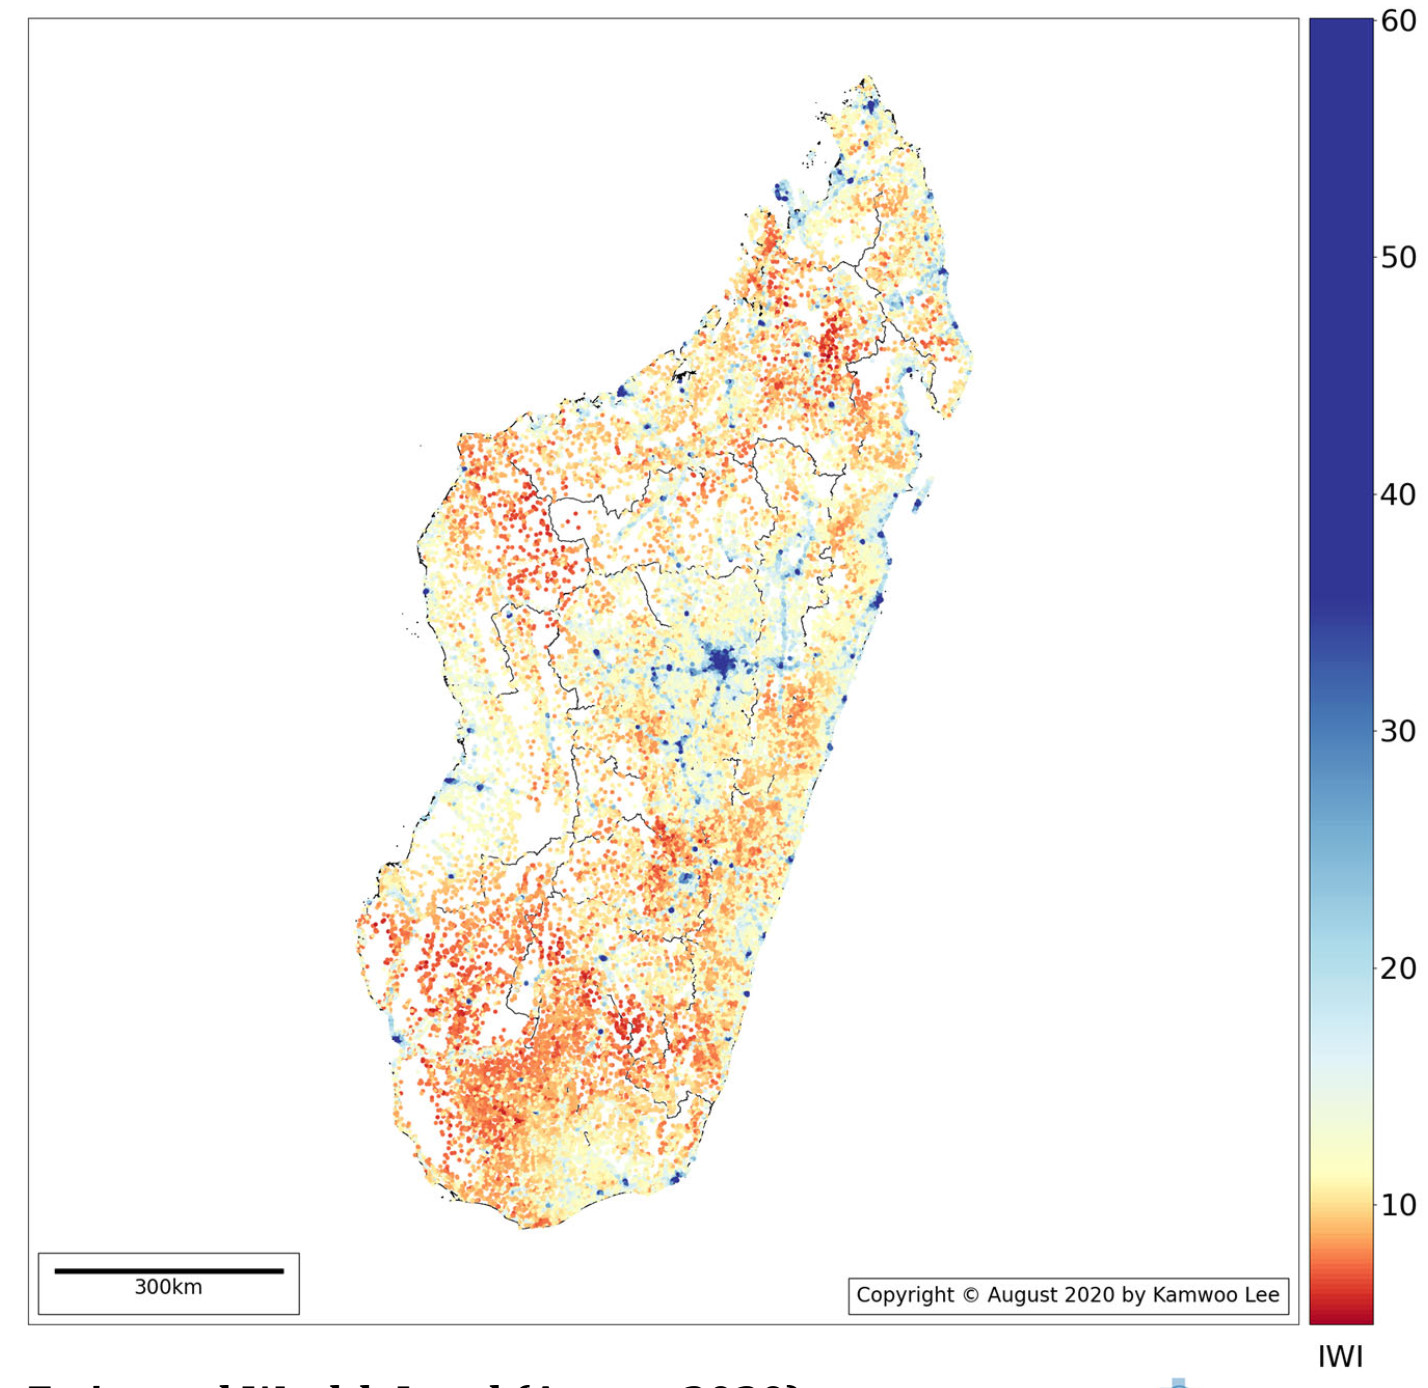
\includegraphics{sources/Poverty_Madagascar.jpg}

\hypertarget{facteurs-favorisant-lessor}{%
\subsection{Facteurs favorisant
l'essor}\label{facteurs-favorisant-lessor}}

\begin{itemize}
\tightlist
\item
  Disponibilité gratuite
\item
  Couverture mondiale, même là où peu d'autres données
\item
  Fréquences de mise à jour
\item
  Accessibilité des infrastructures et systèmes de traitement
\item
  Disponibilité de données pré-processées
\item
  Matériel didactique
\item
  Initiatives de soutien
\end{itemize}

\hypertarget{risques-et-duxe9rives-de-la-popularisation}{%
\subsection{Risques et dérives de la
popularisation}\label{risques-et-duxe9rives-de-la-popularisation}}

\begin{itemize}
\item
  Risque méthodologique : mésusages des données, traitements ou
  interprétation
\item
  Risque épistémologique : métaphore du lampadaire
\item
  Risque sociopolitique : cybertariat, solutionnisme (Fourcade and
  Gordon 2020; Burrell and Fourcade 2021)
\item
  Risque techno-économique : place centrale de Google Earth Engine dans
  ce phénomène
\item
  Economie politique : le terrain à distance
\end{itemize}

\hypertarget{pistes-de-solution}{%
\subsection{Pistes de solution}\label{pistes-de-solution}}

\begin{itemize}
\item
  Plateformes libres et/ou publiques :

  \begin{itemize}
  \tightlist
  \item
    Infrastructures : ex. Copernicus
  \item
    Systèmes: ex. Onyxia (INSEE)
  \item
    Logicielles: ex. Mapme (KfW, AFD)
  \end{itemize}
\item
  Formations et réseaux d'échange
\item
  Approches mixtes incluant qualitatif et terrain
\item
  Réflexivité
\end{itemize}

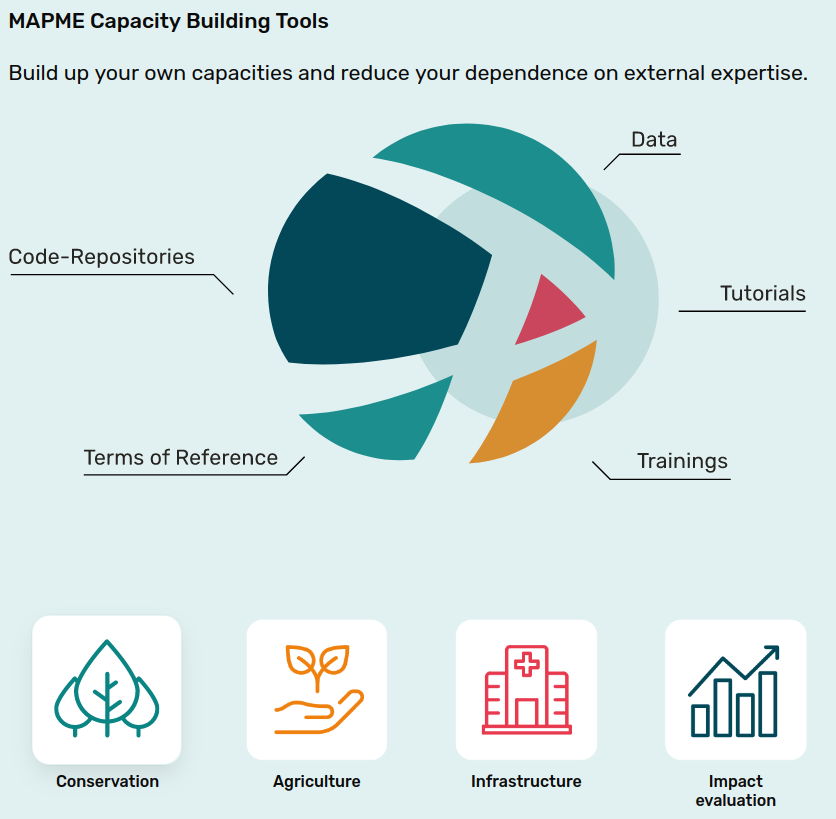
\includegraphics[width=5.20833in,height=\textheight]{sources/Mapme.png}

\hypertarget{ruxe9fuxe9rences}{%
\subsection*{Références}\label{ruxe9fuxe9rences}}
\addcontentsline{toc}{subsection}{Références}

\hypertarget{refs}{}
\begin{CSLReferences}{1}{0}
\leavevmode\vadjust pre{\hypertarget{ref-burrell2021}{}}%
Burrell, Jenna, and Marion Fourcade. 2021. {``The Society of
Algorithms.''} \emph{Annual Review of Sociology} 47 (1): 213--37.
\url{https://doi.org/10.1146/annurev-soc-090820-020800}.

\leavevmode\vadjust pre{\hypertarget{ref-donaldson2016}{}}%
Donaldson, Dave, and Adam Storeygard. 2016. {``The View from Above:
Applications of Satellite Data in Economics.''} \emph{Journal of
Economic Perspectives} 30 (4): 17198.

\leavevmode\vadjust pre{\hypertarget{ref-estoque2020}{}}%
Estoque, Ronald C. 2020. {``A Review of the Sustainability Concept and
the State of SDG Monitoring Using Remote Sensing.''} \emph{Remote
Sensing} 12 (11): 1770.

\leavevmode\vadjust pre{\hypertarget{ref-fourcade2020}{}}%
Fourcade, Marion, and Jeffrey Gordon. 2020. {``Learning Like a State:
Statecraft in the Digital Age.''} \emph{Journal of Law and Political
Economy} 1 (1).

\leavevmode\vadjust pre{\hypertarget{ref-geo2019}{}}%
GEO. 2019. {``EO4SDG: Earth Observations in Service of the 2030 Agenda
for Sustainable Development. Strategic Implementation Plan
2020{\textendash}2024.''} Geneva.

\leavevmode\vadjust pre{\hypertarget{ref-lee2022}{}}%
Lee, Kamwoo, and Jeanine Braithwaite. 2022. {``High-Resolution Poverty
Maps in Sub-Saharan Africa.''} \emph{World Development} 159: 106028.

\end{CSLReferences}



\end{document}
